\section{Technique}
\label{sec:technique}
%
\begin{algorithm}[]
\SetAlgoLined
Input: (symbolic conditional branch instruction inst)\;
$\region_{initial}$ = jit-region-construction(inst)\;
$\region_{no\_return}$ =  return transformation($\region_{initial}$)\;
$\region_{alpha}$ =  alpha-renaming transformation($\region_{no\_return}$)\;
$\region_{before}$ = $\region_{alpha}$\;
$\region_{after}$ = null\;
\Repeat{($\region_{before} = \region_{after}$)}
{
	\Repeat{($\region_{before} = \region_{after}$)}{
		\uIf{($\region_{after} \neq $ null)}
			{$\region_{before}  = \region_{after}$}
		$\region_{sub}$ =  substitution transformation($\region_{before}$)\;
		$\region_{ord}$ =  higher-order transformation($\region_{sub}$)\;
		$\region_{field}$ =  field references transformation($\region_{ord}$)\;
		$\region_{array}$ =  array references transformation($\region_{field}$)\;
		$\region_{simple}$ =  simplification transformation($\region_{array}$)\;
		$\region_{after}$ = $\region_{simple}$\;
		
		}
		$\region_{after}$ =  higher order transformation($\region_{after}$)\;
	}
$\region_{single\_path}$ = single-path cases transformation(R)\;
$\region_{linear}$ = linearization transformation(R)\;
$\region_{green}$ = to-green transformation(R)\;

\eIf{is-canonical($\region_{green}$)}
	{populate outputs \tcp{successful transformation} 
	skip region execution\;}
   {abort \tcp*{resume DSE of conditional branch instruction}}  
   
\caption{Ranger general pseudocode}
\label{fig:algorithm}
\end{algorithm}

\newtext{Algorithm~\ref{fig:algorithm} describes how \tool\ works.
%
The main idea is that \toolshort\ intercepts
conditional branch instructions with symbolic operands and attempts to summarize instructions that lie along
every possible path in the region, up until the program location where all paths in the region merge.
%
We call this summarization a ``region'' or just \region.
%
It is important to note that, \region\ contains not only the summarization in form of a Ranger IR
statement, it also contains other environment-related information, such as types, input and outputs of the region,
explained later in this section.}

\newtext{\tool\ uses Just-In-Time~(JIT) analysis and, with the help of Wala~\cite{Wala},
constructs the control-flow graph~(CFG) of the method containing the intercepted symbolic conditional branch instruction.
%
Then \toolshort\ translates a part of the CFG, that begins from the node containing the symbolic conditional branch
and ends at this node\rq s immediate post-dominator,
into a Ranger IR statement and an environment (line 2). We call this step ``JIT region construction''.}
%
\newtext{The region is said to ``begin'' at the symbolic conditional branch instruction and ``end'' at the address of the first
instruction in the immediate post-dominator of the node that contained the symbolic conditional branch instruction.}

\newtext{Next, \tool\ then runs different transformations on \region\ (lines 2-22) with the goal of reducing the region\rq s
IR statement into a canonical form that can be easily translated into a formula. }

\newtext{These transformations perform operations, like for example inlining method summaries and supporting field
accesses, that will allow the Ranger IR statement to ultimately be translated to a formula.}
%
\newtext{But, dependencies between these transformations are not pre-determined.
%
For example, a region can contain field accesses and a method invocation, the summary of which contains other field
accesses.
%
Using a nested fixed-point computation, \toolshort\ ensures that such dependencies are taken into
consideration.}

\newtext{If the transformations produce a canonical form of the region, then \tool\ adds the canonical region summary
to the path condition, populates the region\rq s outputs, and sets the program counter~(the next instruction to be
executed) to the address of the instruction that is at the beginning of the immediate post-dominator.
%
Otherwise, \toolshort\ aborts and allows DSE to resume execution (lines 23-28).}
%
%%
%To add path merging to SPF, we pre-compute static summaries of multi-path code regions and use them to also precompute summaries of methods.
%%
%Algorithm~\ref{fig:algorithm} describes the core algorithm of \tool\ for using such pre-computed summaries.
%%
%Given a multi-path region summary in Ranger IR~(described in Figure~\ref{fig:grammar}), \tool\
%runs two loops, one nested within the other, up to a fixed point in order to ensure that the type
%used for inlining higher-order method summaries is precise.
%%
%\tool\ ensures such precision of the higher-order region\rq s type because it only inlines methods called using a concrete object
%reference for which type information can be recovered from the region\rq s instantiation environment.
%

In the following sections, we first describe \tool\ grammar then we discuss JIT region construction then
finally we talk about different \toolshort\ transformations and their semantic meaning. We also show how each
transformation is realized on the motivating example presented in Figure~\ref{fig:mot-example}
%
%\begin{figure*}[]
%    \caption{Overview of transformations on Ranger IR to create and instantiate regions up to a fix-point.}
%    \label{fig:overview}
%    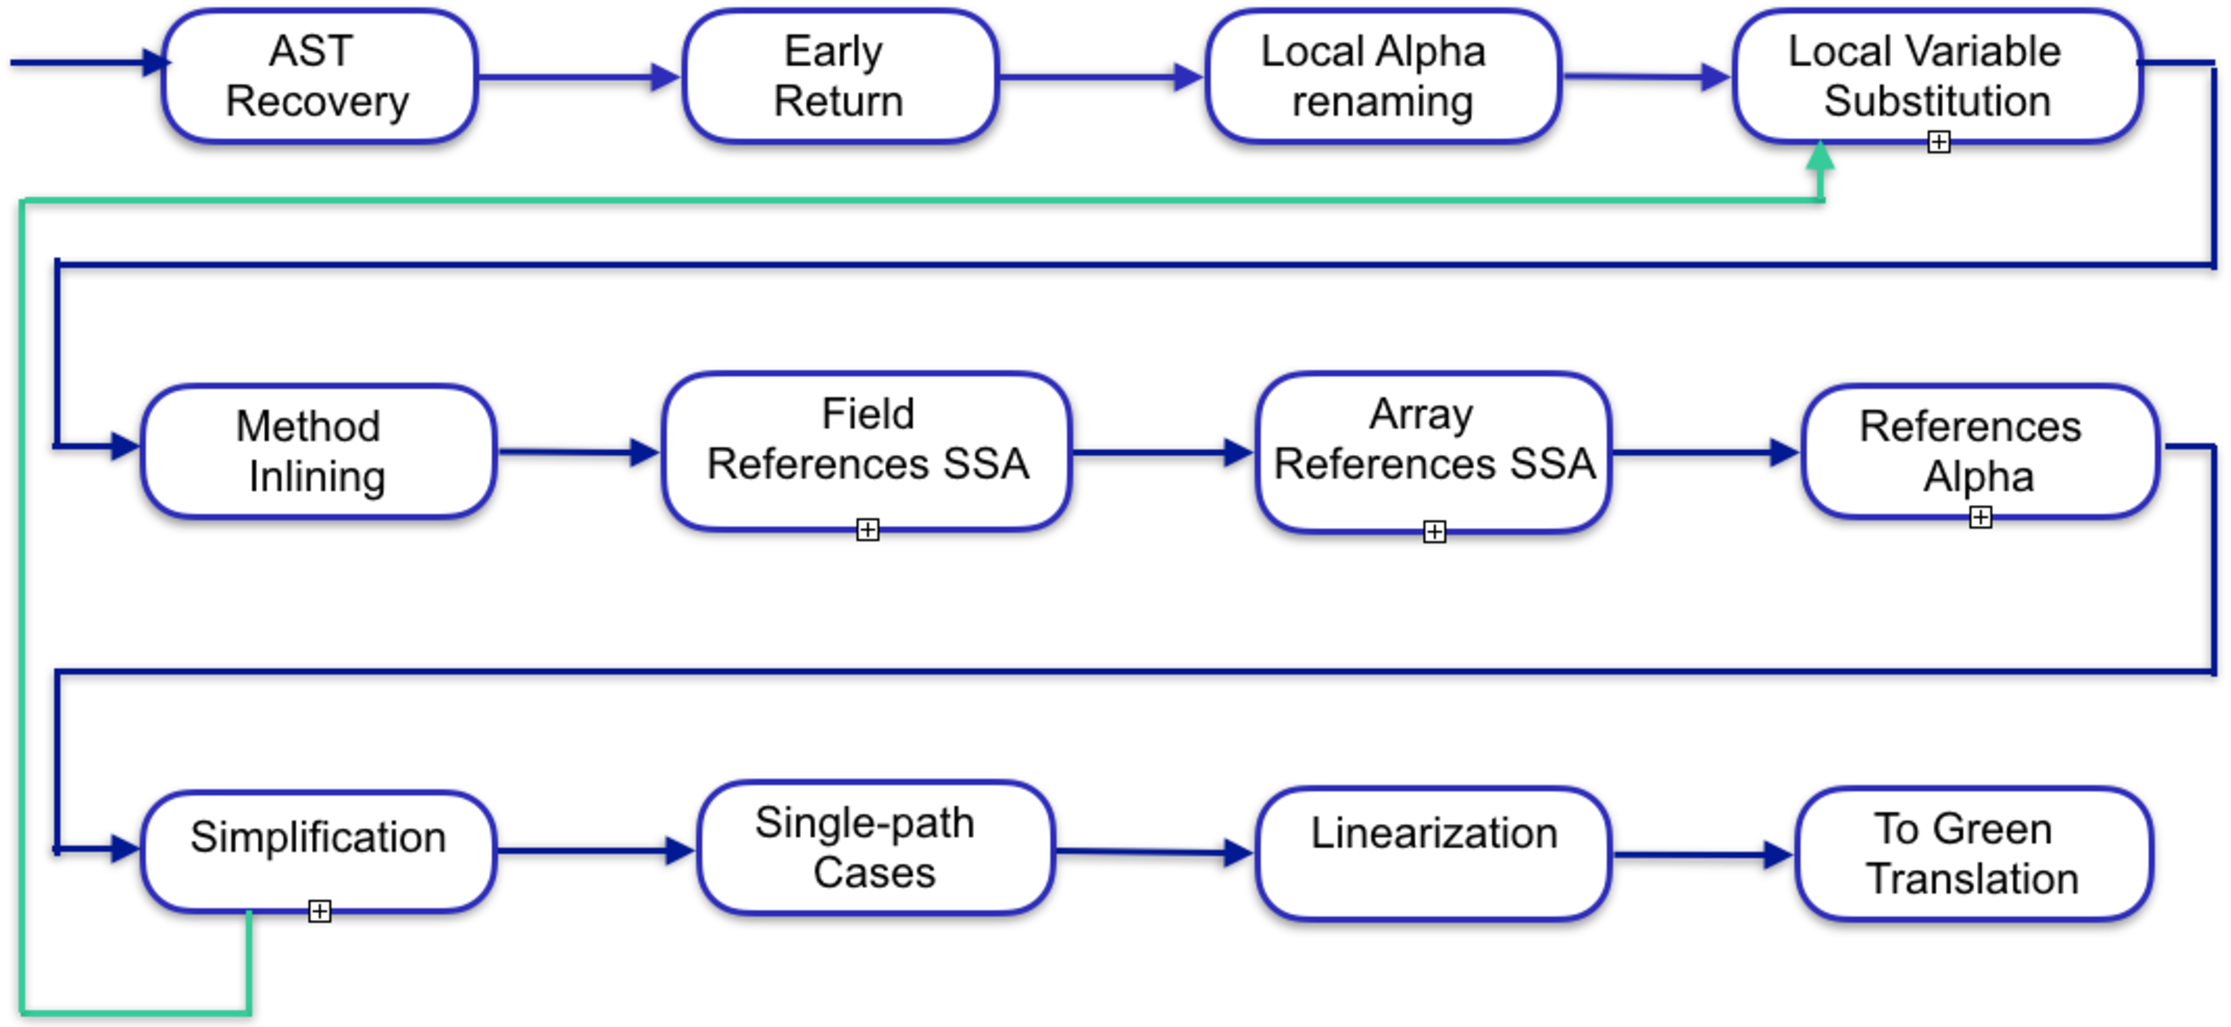
\includegraphics[width=1.5\columnwidth]{figures/transformations.pdf}
%\end{figure*}
%
%
%\subsection{WALA-based analysis for veritesting}
%%
%Veritesting requires static construction of
%predicates of a multi-path region which represent changes to the path expression of the dynamic
%symbolic executor.
%%
%It also requires construction of a control-flow graph of method bodies
%from Java bytecode and finding exit points of the region, which in turn
%requires creation of a control-flow graph of the region.
%%
%Implementing veritesting is made simpler by using a static single
%assignment~(SSA)~\cite{ssa} representation of the multi-path region.
%%
%Using an SSA form allows us to use the $\phi$-expressions created by the
%SSA form and translate them into points at the end of the veritesting
%region where updates to system state along different paths in the region
%can be merged.
%%
%\mike{MWW: Vaibhav please update to describe WALA}
%WALA~\cite{} is a static analysis framework for Java programs that
%has both these features, with
%ExceptionalUnitGraph~\cite{exceptionalunitgraph} and the Shimple
%IR~\cite{shimple}.
%%
%For simple regions with only one exit point, like the one presented in Listing~\ref{lst:v_ex}, we
%were able to use Soot to automate static construction of the predicate representing
%an update to the expression.
%%
%For doing this, we used nodes with more than one successor as the
%starting point, found the immediate post-dominator of the starting
%point, and traversed the control-flow graph on all sides of such branches.
%%
%During such a traversal, we constructed predicates representing the
%multi-path region, similar to the ones presented in
%Listing~\ref{lst:v_ex_smt2}.
%%
%As explained in Section~\ref{sec:exit_points}, including virtual
%function invocations in the construction of our predicates amplifies the
%benefits of veritesting even further.
%%
%We plan to automate this inclusion in the future using Soot.
%%
%Providing SPF with updates to be made to its symbolic store also
%requires Soot to maintain stack location information for variables.
%%
%We plan to automate SPF\rq s symbolic store updates using Soot in the
%future.
%%
%

%\subsubsection{Statement Recovery Setup}
%%
%To bound the set of code regions we analyze, we start by specifying a method $M$ in a configuration file.
%%
%Next, we construct a set containing only the class $C$ that contains $M$.
%%
%We then get another set of classes, $C'$,
%such that every class in $C'$ has at least one method that was called by a method in a class in $C$.
%%
%This step which goes from $C$ to $C'$ discovers all the classes at a class depth of 1 from $C$.
%%
%We continue this method discovery process up to a class depth of 3.
%%
%We found that summarizing
%arbitrary code regions with more than 3 steps deep did not lead to practically useful region summaries.
%%
%Next, we attempt to summarize these methods and regions in them.
%
\begin{figure}
\begin{grammar}
<stmt> ::= <canonical-stmt> | $\lambda$ x.<stmt> 
\alt <stmt> ; <stmt> | <exp> := <exp>
\alt <exit_stmt> | if <exp> then <stmt> else <stmt> 
\alt invoke( <exp>, <exp> )  | exit

<canonical-stmt> ::= <canonical-stmt> ; <canonical-stmt> 
\alt <canonial-exp> := <canonical-exp> | skip

<exit-stmt> ::=  new $\tau$  | return <exp> |  throw <exp> 

<exp>  ::=  <canonical-exp> | get_field( <exp>.<exp> ) 
\alt put_field( <exp>.<exp>, <exp> ) | array_load( <exp>, <exp>) 
\alt array_store( <exp>, <exp>, <exp> ) 

<canonical-exp> ::= <val> | <var> | <canonical-exp> $op_b$ <canonical-exp> 
\alt $op_u$ <canonical-exp> | gamma(<canonical-exp>, <canonical-exp>, <canonical-exp>)

<$op_b$> ::= $+$ | $-$ | $*$ | $\div$ | \& | bitwise-or | $\oplus$ | \% | $==$ | $\neq$ | $\leq$ | $\geq$ | \&\& | logical-or | \textgreater | \textless | $\ll$ | $\gg$ | $\ggg$

<$op_u$> ::= $-$ | \textasciitilde  \quad <val> ::= \unit | $\mathbb{Z}$ |  $\mathbb{C}$ \quad <var> ::= ID_$\mathbb{N}$
\end{grammar}
\caption{Context Free Grammar for Java Ranger IR}
\label{fig:grammar}
\end{figure}


\begin{figure}
$$
\begin{array}{lllll}
\text{Value-maps} & \Delta_r: loc \rightarrow & ( val, exp) &&
\\
& \Delta_s: loc \rightarrow & ( val, exp) &&
\\
\text{Type-maps}  & \Gamma_r: var \rightarrow & \tau & &
\\
& \Gamma_s: ref \rightarrow & \tau&&
\\
\text{Region-map} & \Psi: \tau \rightarrow & \lambda x.s &&
\\
\text{path-subscript-map} & psm: v \rightarrow & x &&
\\
& \Theta: var \rightarrow & loc &&
\\
\text{path-constraints} & \Sigma: \{exp\} &  &  & 
%\\
%\text{Return-constraints} & \Sigma_{ret}: x_{ret} \rightarrow & \exp &  & 
\\
\text{Nominal-next-instruction} & Next: & \mathbb{Z} &  & 
\\
\text{Return-next-instruction} & Next_{ret}: & \mathbb{Z} &  & 
\end{array}
$$
\caption{Environments used in Ranger.}
\label{fig:environment}
\end{figure}

%Java Ranger has its own AST that captures the statement of regions.
%%
%The choice of having a separate AST for Java Ranger, enables the integration of Java Ranger with any static analysis framework by implementing the transformation that transforms the CFG of a given IR into the corresponding Java Ranger AST representation. 
%%
%We call this interface \textit{Statement Recovery} transformation. \\
%%
%In this transformation we visit nodes in topological order by walking normal edges of a branching points until a \textit{minimum convergent node} is encountered. We define a minimum convergent node as the last immediate successor of blocks following a branching node.
%%
%Note that exceptional edges are ignored during this transformation, however exceptional behavior is later identified and handled through the single-Path Cases.
%%
%We discuss more about this in section~\ref{sec:instantiationTransformations}.
%%
%There are two other things that this transformation takes care of: recovering of complex if-then-else and construction of Gated Single Assignment (GSA).
%%
%Recovering of complex conditions in an if-statement restores its form in the source code. 
%% 
%This is done by identifying \textit{immediate self-contained subgraphs}, that is, subgraphs where the initial node is immediately pre-dominated by the initial node and for the static region and whose successor nodes (up to the region terminus) are dominated (not necessarily immediately) by the initial node.
%%
%
%Construction of Gated Single Assignment (GSA) on the other hand is done by keeping track of the current "conditional path" during translation. More precisely this is done by keeping a stack of  {\tt(Expression x enum \{Then, Else\})} pairs. 
%%
%In addition to that, for each edge between blocks in the block structure, the associated "conditional path" is recorded.  
%%
%So the type of this map (the blockConditionMap) is: {\tt(ISSABasicBlock x ISSABasicBlock) --> List of (Expression x enum \{Then, Else\})}.
%%
%Finally creation of the condition of GSA is done during translating a phi-instruction its immediate predecessor blocks are retrieved then we look up  the edges in the blockConditionMap.  From here, and using condition stack leading to that branch, an if/then/else statement is constructed.

\subsection{\tool\ Grammar}
\newtext{Figure~\ref{fig:grammar} shows \tool\ grammar, which can be thought of as a superset of Wala IR which is in turn a superset of Java bytecode instructions. }

\newtext{\toolshort's grammar is composed of statements $stmt$ and
expressions $exp$. Statements include $\langle canonical\text{-}stmt\rangle$ used to describe the simplest form of statements in which different transformations of \toolshort\ tries to reduces to. A region statement $\lambda x.\langle stmt \rangle$, which defines the binding of the input parameter in the region statement. Other statements in \toolshort\ IR also include: sequential composition ($stmt ; stmt$), assignment ($exp := exp$),
skip, exit ($exit\text{-}stmt$) (which determine single-path Cases, it includes $new\; \tau$, $throw\; exp$ and $return\; exp$ statements), if-then-else and finally $invoke$ statement to indicate call of a method.}

%In the following sections we will discuss the various parts of this statement to show the effect of various transformations.
%
%It consists of different kinds of statements of which
%$exit$ statements define single-path cases present in the region and $skip$ statements allow simplifications to
%reduce the size of the region summary.
%Statements in Java Ranger contains: sequential composition ($stmt;stmt$), assignment ($exp = exp$), a
%skip, parametric statements $x.stmt$, exit-statements $exit$, which determine single path regions and they are $new\;
%\tau$, $throw\; exp$ and $return\; exp$, if-then-else, method invocation $invoke(exp, exp, exp)$ and especial $exit$
%statement to bookmark exit point of a region/statement.
%


\newtext{\toolshort\ expressions consist of $\langle canonical\text{-}exp\rangle$, which is analogous to canonical statements, which describes the simplest form of expressions that \toolshort\ tries to reduce to.  $\langle canonical\text{-}exp\rangle$ includes constants aka values (unit \unit, positive and negative integers $\mathbb{Z}$, characters $\mathbb{C}$), variables (these are subscripted with integers to facilitate having SSA form for them
ID_$\mathbb{N}$), binary and unary operations over canonical expressions as well as a special gamma expression, $gamma(exp, exp, exp)$. Gamma expression that allow Ranger IR to construct Gated Single Assignment~(GSA)\cite{} form for variables which intuitively describes conditional assignment of variables.}

\newtext{Java Ranger defines 4 types of variables, a field or array variable (created to maintain fields and arrays ssa), a return variable (to carry the return values), variables that correspond to local variables, and variables used
to represent intermediate computation. This distinction is abstracted away from the grammar but is referred to whenever necessary in the text.
}

\newtext{Other forms of expressions include non-canonical expressions, this includes read and writes to fields and arrays. }
%
%
%Java Ranger expressions on the other hand are: values (unit \unit, positive and negative integers $\mathbb{Z}$ and
%characters $\mathbb{C}$) , variables (these are subscripted with integers to facilitate having ssa form for vars
%D_$\mathbb{N}$), binary operations $op_b$, unary operations $op_u$,  $get-field(exp)$ and $put-field(exp, exp, exp)$ for
%accessing and changing fields,  $array-load(exp)$ and  $array-store(exp, exp, exp)$ for accessing and changing array
%elements, a special gamma expression, $gamma(exp, exp, exp)$, that operates like $?:$ in Java. Gamma expression are
%fundamentally important to Java Ranger because it is how Java Ranger determines the conditions of different paths as
%well as the evaluation of variables along these paths. It worth pointing out that Java Ranger defines 3 types of
%variables, a field or array variable (created to maintain fields and arrays ssa), an early return variable (to carry
%early return values) and any other type of variables. We assume the existence of a special function $gen_var$ that would
%generate one variable in the right sequence for each of these types.
%
%We assume the existence of a special function $gen\_var$ that would generate one variable for each of these types.
%
%In the remaining sections we will use $x$ to refer to a Ranger IR variable, $x_{ref}$ to refer to variables constructed for
%fields and arrays and $x_{ret}$ for variables constructed for early return construction.
%
%Similarly we will use $s$ to refer to statements, $e$ to refer to expressions and $v$ to refer to values.


\subsection{JIT Region Construction}
\label{sec:jit}
\newtext{The construction of a region happens when \tool\ detects a symbolic conditional branch
during DSE, and thus an opportunity for path-merging. Using the recovered cfg of the method where the intercepted
conditional branch instruction resides, \toolshort\ constructs two types of regions: \textit{multi-path region} and \textit{method-region}.}

\newtext{A \textit{multi-path region} contains a statement in \toolshort\ IR and a corresponding environment. The IR
statement represents the summarization of the instructions from the conditional instruction basic block, i.e,
if-bytecode basic block, and down until the merge point, i.e, the phi basic block. The region environment that contains
information about variables in the region, such as types of variables, variables stack slot information, inputs of the
region and output of the region.}

\newtext{A \textit{method-region}: also contains a statement in \toolshort\ IR and an environment. This time however the
IR statement represents the summarization of the whole method. The environment for a method-region is similar to
the multi-path region, except that the input and the stack slot of variables are defined in terms of the parameters to
the method.}

\newtext{In the next subsections we describe the two main steps in constructing a region, the IR statement creation,
which we call \textit{IR statement recovery} and the environment creation for regions.}
\subsubsection{IR Statement Recovery}
%In this step, a Java Ranger is created from the corresponding CFG. Since regions of interest for our technique are
%bounded by the branch and meet of a given acyclic subgraph.  The intuition is that path explosion during execution of
%loops is driven by conditional logic within the loop, rather than the loop itself. %Starting from an SSA form, the first
%transformation recovers a tree-shaped AST for the subgraphs of interest.  While this step is not strictly necessary, it
%substantially simplifies subsequent transformations.
%
In this step, we recover the Ranger IR of a region from its Java bytecode representation.
%
While the Java bytecode operaters as a register~(used for local variables) and stack~(used for instruction operands)
machine, the Ranger IR captures the region in Static Single Assignment~(SSA) form with inputs corresponding to
local variables and outputs corresponding to local variables or the stack.
%
The algorithms used in this step are similar to those used for decompilation~\cite{Yakdan15@decompilation}. % but with slightly different goals:
%\begin{itemize}
%    \item The algorithm must be {\em accurate} but need not be {\em complete}.  That is, obfuscated regions of code need not be translated into a tree form.
%    \item The algorithm must be {\em lightweight} in order to be efficiently performed during analysis.  Thus, algorithms that use global fixpoint computations are
%        too expensive to be used for our purposes.
%\end{itemize}
%
Starting from an initial basic block in a control-flow graph recovered by Wala~\cite{Wala}, the algorithm first finds
the immediate post-dominator of all {\em normal} control paths, that is, paths that do not end in an exception or return
instruction.
%
It then looks for nested self-contained subgraphs.
%
If for any graph, the post-dominator is also a predecessor of the node, we consider it a loop and discard the region.
%
The algorithm systematically attempts to build regions for every branch instruction, even if the branch is already
contained within another region.
%
The reason for this is that, it may not be possible to instantiate the larger region depending on whether summaries can be found
for {\em dynamically-dispatched} functions, and whether references are {\em uniquely determinable} for region outputs.
%
The outcome of this step is a statement in \tool.
%
This step does not compute loop summaries, it does summarize regions contained before, within, and after loops.
%
For region 2 shown in the motivating example in Figure~\ref{fig:mot-example}, the recovered statement is as follows where
$x58$ corresponds to input from $inWord$, and $x54$, $x55$ correspond to outputs to $wordCount$,
$inWord$ respectively.\\
%
\begin{lstlisting}[numbers=none]
if ((! (== x58 0 ) )) {
  x44 = invokeinterface < Application, Ljava/util/List, get(I)Ljava/lang/Object; >[x9,x59]
  x47 = invokevirtual < Application, Ljava/lang/Integer, intValue()I > x44
  if ((! (!= x47 0 ) )) {
    x48 := (+ x57 1 );
  }
} else { ... }
x54 := (Gamma !(x58==0) (Gamma !(x47!=0) x48 x57) (Gamma !(x53==0) x57 x57));
x55 := (Gamma !(x58==0) (Gamma !(x47!=0) 0 x58) (Gamma !(x53==0) 1 x58));

\end{lstlisting}
%\ref{lst:walk_static}.
\subsubsection{Environment Creation}

\newtext{Once the statement of a region has been recovered, i.e., a corresponding \toolshort\ IR statement has been created, \toolshort\ then tries to populate its corresponding environment.}
%
This includes identifying the region boundary, in terms of the region\rq s local variable inputs and outputs, types, and stack
slots of variables used in the region summary.
%
%The region boundary is used to identify boundaries of the region w.r.t local variables.
%
%This is used later to constrain the computation and population of Ranger IR environment tables.
%

\newtext{\toolshort\ defines local variable inputs as variables in the region summary that make the first \textit{use} of a
given stack slot. This is called an input variable(s) to the region because, when the DSE hits a symbolic region where there is a opportunity of path-merging, \toolshort\ collects information (concrete/symbolic values) from the dynamic environment of DSE, and substitute them in the region's statements, i.e, substituting the first binding of variables to a stack slot with its actual concrete or symbolic value. Using these environment-related information \toolshort\ continue trying to either dereference objects used in the IR statement or express them in a canonical form. }
%

\newtext{Similarly, local variable outputs are the last \textit{def} of a \toolshort\ IR variable in a region summary that maps to a given
stack slot. \toolshort\ uses this information to populate symbolic expression or concrete values that summaries the execution of the region.}
%The output table is populated with the last \textit{def} of a local variable at merge point of the region.
%
%We also use local variable type information for all variables that lie within the boundary of the region.
%
%this is initially done by inquiring the static analysis framework, WALA~\cite{Wala} but is later changed by inferring types of local variables
%at instantiation and during type propagation transformation~\ref{sec:instantiationTransformations}.
%We infer type information using the instantiation environment of a region for local variables, field references, and
%array references.
%
\newtext{To do this, \toolshort\ relies on Wala to provide stack slot information for intermediate variables. This is however not always available and therefore \toolshort\ needs to try to infer the mapping of intermediates to stack slots. This is done using the observation that, if at one variable used in a $\phi$-expression of Wala maps to a stack slot, then all variables
used in that $\phi$-expression must belong to the same stack slot.
%
\toolshort\ use this observation to propagate stack slots across all $\phi$-expressions. 
}
%Again, we use the dynamic environment to map \toolshort\ IR variables to their corresponding stack slots, starting with
%the stack slot information provided by Wala. However, 
%We also construct a stack slot table as part of a region\rq s Ranger IR summary.
%
%The stack slot table maps Ranger IR variables to a stack slot, if they correspond to a local variable in the source code.
%
%We populate the stack slot table by obtaining a variable to stack slot mapping from WALA.
%
%We also assume that, if at least one variable used in a $\phi$-expression of Wala maps to a stack slot, then all variables
%used in that $\phi$-expression must belong to the same stack slot.
%%
%We use this assumption to propagate stack slots across all $\phi$-expressions.
%
%

Formally we define the following structures:\\
%
\textbf{Value-map}: $\Delta_r$ and $\Delta_s$ maps a location (i.e, stack slots, heap entry), to concrete $val$ or symbolic $exp$ for Java Ranger and DSE respectively. This is used to collect the input of the region as well as to populate the output of the region.\\
\textbf{Type-map}: $\Gamma_r$ and $\Gamma_s$ maps vars or references, to types $\tau$ for Java Ranger and DSE respectively.\\
\textbf{Region-map}: \tool\ defines a map $\Psi$ from type $\tau$  to a parametric statement $\lambda x.s$ that defines the region\rq s summary. \newtext{This is used to bind the region type to its statement. The actually form of the region type is abstracted here, but really it is defined by class-name, method-name and instruction line number. This way, if a region is every hit again, i.e., executed again, then instead of re-running the jit-region construction, \toolshort\ just pulls the region from the map.}\\
\textbf{Path-Constraint-List}: A list $\Sigma$ of path constraints. \newtext{This is later used to guide the DSE execution to particular paths that \toolshort\ did not summarize, more information is in next section.}\\
%\textbf{Return-Constraint-map}: A map $\Sigma_{ret}$ from return vars $x_{ret}$ to return constraints. \newtext{This is used to set up the path condition for return case, more information is in next section.}
\newtext{\textbf{Nominal-next-instruction}: is a the instruction position that DSE should resume from, if path-merging was successful.}
\newtext{\textbf{Return-Next-instruction}: is a the instruction position that DSE should resume from, if path-merging was successful for return case.}


Figure~\ref{fig:semantics} shows the semantics of different transformations, where the judgment describes a transformation step on some statement s, w.r.t. the maps, which usually yield a new statement $s'$ and possibly some changes in the map.\\
%
%The stack slot table on the other hand, does not use region boundary for its population. The reason for this is that,
%the static analysis framework we use, WALA, sometime does not provide information about the stack slots of intermediate
%variables.
%%
%This is particularly problematic in our case because the def of a phi is both an intermediate variable, and so we do
%not know its stack slot, yet it is also an output of the region for which we want to populate its symbolic
%representation onto the stack slot.
%%
%Therefore, our stack slot table uses stack slot inference by propagating the stack slots of vars used in a phi onto the
%def of the phi.
%%
%This requires visiting all variables and phi statements of the IR to maximize the inference of the stack slot, this is
%repeatedly done until a fix point is reached.
%
\begin{figure*}[t]
    \footnotesize
\fbox{%
\parbox{0.98\textwidth}{%
%$$
%\infer[\rn{early-return_1}]
% {\step{\Sigma_{ret}}{\ifr{e_1}{s_1}{(s_2 ; \return{e_2})}}{\Sigma_{ret} \cup (x_{ret}, e_2)}{(\ifr{e_1}{(s_1 ; \return{e_2})}{s_2}) ; x_{ret} := e_2}{}}
% {gen\_id() = x_{ret} \qquad \text{no_return}(s_1) \qquad \text{no_return}(s_2)}
%$$
%$$
%\infer[\rn{get-return_2}]
%{\step{\Sigma_{ret}}{\ifr{e_1}{s_1}{s_2}}{\Sigma_{ret}\cup (x_{ret},(e_1\wedge c_1)\vee( e_1 \wedge c_2))}{(\ifr{e_1}{s_1}{s_2}) ; x_{ret} = gamma((c1 \wedge e_1), e_1',  e_2')}{}}
%{\step{\Sigma_{ret}}{s_1}{\Sigma_{ret}\cup (w1_{ret},c_1)}{s_1' ; w1_{ret} := e_1''; \return e_1'}{}  \qquad
%\step{\Sigma_{ret}}{s_2}{\Sigma_{ret}'\cup(w2_{ret}, c_2)}{s_2' ; (w2_{ret} := e_2'' ; \return e_2')}{} \qquad gen\_id() = x_{ret}}
%$$

$$
\infer[\rn{get-return}]
 {\step{\Sigma}{\ifr{e}{(s_1; \return{v_1})}{s_2}}{\Sigma}{(\ifr{e}{s_1; \return{v_1}}{s_2}) ; x_{ret} = v_1}{}}
{
Next = position(if_{inst}.next())
\qquad
Next_{ret} = position(return_{inst})
\qquad
gen\_id() = x_{ret}}
$$

$$
\infer[\rn{substitution}]
 {\step{\Theta, \Delta_s}{\lambda x.s}{\Theta, \Delta_s}{\sub{(v,e)}{x}{s}}{sub}}
 {\lookup{\Theta}{x} = l , \qquad \lookup{\Delta_s}{l}=(v,e)}
\qquad
\infer[\rn{to-green}]
 {\step{\Sigma}{x := gamma(e_1, e_2, e_3)}{\Sigma}{( e_1 \wedge x = e_2) \vee ( !e_1 \wedge x = e_3)}{}}
 {}
$$
$$
\infer[\rn{high-order}]
 {\step{\Gamma_r, \Delta_r}{s_1; invoke(e_1, e_2, e_3)}{(\Gamma_r \cup \Gamma_r'), \Delta_r''}{s_1; \sub{v_2}{x}{s_2}}{high}}
 {\step{\Gamma_r, \Delta_r}{e_1}{\Gamma_r, \Delta_r'}{v_1}{sub} \qquad \lookup{\Gamma_s}{v_1.e_2} = \tau , \qquad \Gamma_r', \lookup{\Psi}{\tau}=\lambda x.s_2, \qquad \step{\Delta_r'}{e_3}{\Delta_r''}{v_3}{sub}}
$$
%$$
%\infer[\rn{high-order_2}]
% {\step{\Gamma_r, \Delta_r}{e = invoke(e_1, e_2)}{(\Gamma_r \cup \Gamma_r'), \Delta_r''}{\sub{v_2}{x}{s} ; e = e'}{high}}
% {\step{\Gamma_r, \Delta_r}{e_1}{\Gamma_r', \Delta_r'}{v}{sub}, \qquad \lookup{\Gamma_s}{v} = \tau, \qquad \Gamma_r', \lookup{\Psi}{\tau}= \lambda x.(s; \return{e'}) \qquad \step{\Delta_r'}{e_2}{\Delta_r''}{v_2}{sub}}
%$$
$$
 \infer[\rn{single-path_1}]
 {\sstep{throw \:e}{single}{exit}}
 {}
\qquad
\infer[\rn{single-path_2}]
 {\step{\Sigma}{\ifr{e}{(s_1 ; exit ; s_1' )}{s_2}}{(\Sigma \vee e)}{s_2}{}}
 {}
%\qquad
%\infer[\rn{single-path_3}]
% {\step{\Sigma}{\ifr{e}{s_1}{(s_2 ; exit ; s_2')}}{(\Sigma \vee !e)}{s_1}{}}
% {}
%$$
%$$
%\infer[\rn{single-path_4}]
% {\step{\Sigma}{\ifr{e}{(s_1 ; exit ; s_1' )}{s_2 ; exit ; s_2'}}{(\Sigma \vee true)}{skip}{}}
% {}
% \qquad
%\infer[\rn{linearlization}]
% {\sstep{\ifr{e}{s_1}{s_2}}{\compose{s_1}{s_2}}{}}
% {}
$$
%$$
%\infer[\rn{get-field_1}]
% {\step{psm}{x := get\text{-}field(e)}{psm}{ x := (v,e')}{field}}
% {\step{psm}{e}{psm}{v}{any} \quad \Theta(v) = l \qquad \Delta_s (v )=(v,e') \qquad psm(v) = \phi}
%\qquad
%\infer[\rn{get-field_2}]
% {\step{psm}{x := get\text{-}field(e)}{psm}{ x := x_r}{field}}
% {\step{psm}{e}{psm}{v}{any} \qquad psm(v) = x_r}
%$$
$$
\infer[\rn{put-field_1}]
 {\step{\Gamma_r, psm}{x := put\text{-}field(e1, e2)}{(\Gamma_r \cup (x_0, \Gamma_s{v})), (psm\cup(v, x_0))}{ (x := x_0); (x_0 := e2)}{field}}
 {\step{\Gamma_r, psm}{e}{\Gamma_r, psm}{v}{any} \qquad \Theta(v) = l \qquad psm(v) = \phi }
$$
$$
\infer[\rn{put-field_2}]
 {\step{\Gamma_r, psm}{x := put\text{-}field(e1, e2)}{(\Gamma_r \cup (x_{ref}', \Gamma_r(x_{ref}))), (psm\cup(v, x_{ref}'))}{ (x := x_r) ; (x_{ref}' := e2)}{field}}
 {\step{psm}{e}{psm}{v}{any} \qquad \Theta(v) = l \qquad psm(v) = x_{ref} \quad gen\_id() = x_{ref}'}
$$
$$
\infer[\rn{gamma-generation_1}]
 {\step{\Gamma, psm}{\ifr{e}{s_1}{s_2}}{\Gamma''), psm''}{\ifr{e}{s_1'}{s_2'} ; x_{ref} = create\text{-}gamma(s_1', s_2', psm)}{field}}
 {\step{\Gamma, psm}{s_1}{\Gamma', psm'}{s_1'}{field} \qquad 
 \step{\Gamma', psm'}{s_2}{\Gamma'', psm''}{s_2'}{field}  \qquad gen\_id() = x_{ref}}
$$
%$$
%\infer[\rn{early-return_3}]
% {\step{\Sigma_{ret}}{\ifr{e}{(s_1 ; \return{e_1})}{(s_2 ; \return{e_2})}}{\Sigma_{ret} \vee true}{\ifr{e}{(s_1 ; \return{e_1})}{skip} ; x_{ret} := e_1}}
% {gen\_id() = x_{ret}}
%$$
}}
\caption{Subset of the Evaluation Rules for Ranger Transformations}
\label{fig:semantics}
\end{figure*}
%
\subsection{Transformations}
\label{sec:Transformations}

\newtext{\textbf{Return Transformation}: In this transformation, Java Ranger converts multi-path region with \textit{one or more} return statements or a method region with \textit{more than one} return statement, into region that assigns a return variable $x_{ret}$  $gamma$ expression that evaluates to different return values depending on the return value predicated on the condition that would cause that value to be returned.}
%
\newtext{The $\rntext{return}$ describe the semantics of this transformation when the return statement is on one side of a multi-path region. In this case \toolshort\ generates a new return variable $x_{ret}$ and assign it to the return variable. Eventually if the path-merging of this region was successful \toolshort\ will in this case generate two paths one to explore the return choice and another to explore the nominal choice. Accordingly, the position where DSE needs to resume from needs to be changed depending on which choice is being executed.}
%
%In this transformation, Java Ranger collects that conditions for branches that
%have early return in them. In figure~\ref{fig:semantics} we show the rule of having an early return on the else side
%$\rn{early-return_1}$ where neither inner statements $s_1$ or $s_2$ are conditional with early return. In this case, the
%statement is transformed to appending an assignment statement to the early return result to a new early return var
%$x_{ret}$, also the condition under which the early return value occurs is added to the early return environment
%$\Sigma_{ret} \cup (x_{ret}, e_2)$
%
%Rule $\rn{early-return_2}$ describes the situation where both the statements $s1$ and $s2$ contains inner conditions
%with early return statements. In this case a new result variable is created $x_{ret}$ and assigned to the gamma
%expression $x_{ret} = gamma((c1 \wedge e_1), e_1',  e_2')$ describing conditions and values assigned under them. In
%addition the context of early return variables-conditions is updated.

\textbf{Alpha-renaming Transformation}: In this transformation, all Ranger IR variables are renamed by adding a subscript
unique to each instantiation of the region.
%
This transformation helps distinguish variables across multiple instantiations of the same region.
%
% This is particularly important not only to ensure uniqueness of variables among different regions, but also to ensure
%uniqueness of variable names of the \textit{same} region whichmight be instantiated multiple times on the same path,
%i.e., a region inside a loop will be instantiated multiple times.
%
%We do not define this transformation formally due to space, but it is basically straight forward by generating a unique
%prefix for each variable and updates the new name in the statement as well as all the contexts in which it appears.
To give an example of this transformation, line 2 in the recovered Ranger IR statement gets changed to:
\begin{lstlisting}[numbers=none]
x44$2 = invoke < Application, Ljava/util/List, get(I)Ljava/lang/Object; >[x9$2, x59$2]
\end{lstlisting}

\textbf{Local Variable Substitution Transformation}: During this transformation, local variable inputs in \toolshort\ are substituted with their concrete or symbolic values obtained from the environment of DSE.
%
\newtext{The $\rntext{substitution}$ rule in Figure~\ref{fig:semantics} describes the semantics of this transformation where the location of an input variable $l$ is used to lookup its value in the DSE environment $\Delta_s$ and is substituted in the region statement.}
%
%The $\rn{substitution}$ given a parametric statement $x.s$, and if $x$ was mapped to a location $l$ then its
%dynamic, i.e., concrete or symbolic $(v, e)$, substitute $x$ in $s$.
Running this transformation on the previous Ranger IR statement causes $x9\$2$ to be
resolved to a concrete integer value 375 to change the statement to %$x44\$2= invoke(ArrayList.get(I)Ljava.lang.Object,375, x59\$2);$\\
%transformation, thus line 2 becomes:
\begin{lstlisting}[numbers=none]
x44$2= invoke(ArrayList.get(I)Ljava.lang.Object,375, x59$2);
\end{lstlisting}
%
\textbf{Higher-order Regions Transformation}: This transformation is initiated when a method invocation after local variable substitution.
%
At this point, we perform three steps.
%
\newtext{(1) The called method\rq s region is retrieved, depending on the dynamic type obtained from DSE, if the region is not found then JIT-region construction is called for it. If a method region was finally constructed/retrieved then its variables are alpha-renamed.}
%
\newtext{(2) For concrete object references that \toolshort\ was able to substitute for callee objects (if it is non-static invocation, otherwise no object reference is need), \toolshort\ uses expressions of IR parameters to substitute the formal parameters by repeatedly applying local variable substitution transformation over the method region.}
%
(3) When no more higher-order method summaries can be inlined, the resulting substituted method region is inlined into
the outer region.
%
%Rules $\rn{high-order}$ and $\rn{high-order_2}$ describe the semantics of this transformation.
%Formally, rules $\rn{high-order_1}$ describes the inlining process for methods that has no return values for a concrete
%reference, 

\newtext{Rule $\rntext{high-order}$ describes inlining of methods that have a single return values for concrete
object reference. In this rule, $e_1$ reduces using substitution to a concrete reference $v_1$ type, then using the DSE environment method-region $\lambda x.s_2$ is pulled out from region map $\Psi$. Finally inlining of the method-region is down where values $v_3$ substitute formal parameters.}
%For non-concerete reference, and after reaching a fixed point, the updated type table (using type
%propagation) is used to get the type of the variable and therefore the corresponding parametric region statement. It
%must be noted that methods with multiple returns, should have been normalized out with the early-return transformation
%discussed previously. Note the rules describes the support for the jvm invoke virtual instruction, however Java Ranger
%supports as well invoke static and invoke interface.

%For $\rn{high_order-1}$ initially after evaluating the reference of the invoke by either finding it concerte value
%through substitution or obtaining it from the updated type table, the type is used to retrieve the parametric region for
%the method being invoked. Substitution of the parameters then follows and direct inlining occurs. In rule
%$\rn{high-order_2}$, inlining of the return value translates to an assignment statement.
%
To show the effect of this transformation on the motivating example, regions that defines
$ArrayList.get(I)java.lang.Object$ are inlined in the original region to get the following Ranger IR statement.
%
Please note that $x58$ from the originally recovered static summary has been substituted by $x40\$1$ because it was
read as a local variable input~($inWord$)~that had the symbolic value $x40\$1$ (a consequence of summarizing region 1 in
Figure~\ref{fig:mot-example}).
%
\begin{lstlisting}[numbers=none]
if ((! (== x40$1 0 ) )) {
  x4$4 = get(375.< Primordial, Ljava/util/ArrayList, size, <Primordial,I> >)
  if ((! (< 0 x4$4 ) )) {
    Throw Instruction
  }
  x4$5 = get(375.< Primordial, Ljava/util/ArrayList, elementData, <Primordial,[Ljava/lang/Object> >)
  x5$5 = x4$5[0:<Primordial,Ljava/lang/Object>]
  x6$3 = x5$5;
  x44$2 = x6$3;
  [x47$2] = invoke < Application, Ljava/lang/Integer, intValue()I >[x44$2]
   if ((! (!= x47$2 0 ) )) {
      x48$2 = (+ 0 1 );
   }
} else { ... }
x54$2 := (Gamma !(x40$1==0) (Gamma !(x47$2!=0) x48$2 0) (Gamma !(x53$2==0) 0 0));
x55$2 := (Gamma !(x40$1==0) (Gamma !(x47$2!=0) 0 x40$1) (Gamma !(x53$2==0) 1 x40$1));
\end{lstlisting}
 
\textbf{Field References SSA Transformation}: This transformation translates reads and writes of fields
in Java bytecode into corresponding Ranger IR statements.
%
In order to translate all field accesses to SSA form, this transformation creates a summary of the semantics
represented by the field accesses in the region.
%
This transformation constructs a new field access variable for every field assignment on every path within the region.
%
This new field access variable construction makes use of two monotonically increasing subscripts.
%
It uses a path subscript to distinguish between assignments to the same field on the same execution path.
%
It uses a global subscript to distinguish between assignments to the same field across execution paths.
%
At the merge point of the region, field assignments done on the same field are merged using
Gated Single Assignment (GSA)~\cite{Ottenstein1990}.
%

\newtext{Rule $\rntext{put-field_1}$ and $\rntext{put-field_2}$ describes the operation of the field transformation over a put-field instruction and rule $\rntext{gamma-generation_1}$ describes the generation of a gamma expression for field SSA vars. The first rule describes a put-field for a concrete reference $v$ that has not been mapped to SSA variable. In this case, \toolshort\ gives a new var with initial subscript $x_0$ and adds that to the $psm$ map.  The second rule describes a situation where the reference has an occurance in $psm$ map, and therefore a new subscript variable is being created $x'_{ref}$ that would be assigned the put field value. Finally the $\rntext{gamma-generation}$ rule, describes the situation where on different sides of an if instruction $psm$ had different subscripted variables appear for the same referenced variable, in this case \toolshort\ creates a gamma statement. }

%
To continue expanding the motivating example, the field references transformation on the above Ranger IR statement
changes the assignments to $x4\$4$ and $x4\$5$ to assign them the concrete values 200 and 397 respectively.
%\begin{lstlisting}[numbers=none]
%if ((! (== x40$1 0 ) )) {
%  x4$4 := 200;
%  if ((! (< 0 x4$4 ) )) {
%    Throw Instruction
%  }
%  x4$5 := 397;
%  x5$5 = x4$5[0:<Primordial,Ljava/lang/Object>]
%  x6$3 := x5$5;
%  x44$2 := x6$3;
%  x45$2 = checkCast(x44$2,[<Application,Ljava/lang/Integer>])
%  [x47$2] = invoke < Application, Ljava/lang/Integer, intValue()I >[x45$2]
%  if ((! (!= x47$2 0 ) )) {
%      x48$2 := (+ 0 1 );
%  }
%} else { ... }
%x54$2 := (Gamma !(x40$1==0) (Gamma !(x47$2!=0) x48$2 0) (Gamma !(x53$2==0) 0 0));
%x55$2 := (Gamma !(x40$1==0) (Gamma !(x47$2!=0) 0 x40$1) (Gamma !(x53$2==0) 1 x40$1));
%\end{lstlisting}
%
Since Java Ranger runs a simplification transformation (which has constant propagation and if-then-else statement
simplification) within the same fixed point iteration, this Ranger IR statement is simplified to the following statement.
%
Please note that the simplification transformation sets variables assigned to a constant value in a constant values
map maintained in the region\rq s instantiation environment.
%
%This causes the assignment to $x48\$2$ to be removed from the below Ranger IR statement and
This causes uses of $x48\$2$ to be substituted by the constant 1.
%
\begin{lstlisting}[numbers=none]
if ((!= x40$1 0 )) {
  x5$5 = 397[0:<Primordial,Ljava/lang/Object>]
  x45$2 := x5$5;
  [x47$2] = invoke < Application, Ljava/lang/Integer, intValue()I >[x5$5]
} else { ... }
x54$2 := (Gamma x40$1!=0 (Gamma x47$2==0 1 0) 0);
x55$2 := (Gamma x40$1!=0 (Gamma x47$2==0 0 x40$1) (Gamma x53$2!=0 1 x40$1));
\end{lstlisting}
\textbf{Array References SSA Transformation}: This transformation translates reads and writes of arrays in
Java bytecode into corresponding Ranger IR statements.
%
In order to translate all array accesses to SSA form, this transformation creates an execution path-specific copy of
every array when it is first accessed within a region.
%
Reads and writes of arrays are then done on a path-specific copy of the array.
%
All array copies are merged at the merge point of multi-path regions.
%
The merged array copy represents array outputs of the region.
%
The effect of this transformation on the last shown Ranger IR statement produces the following statement where the
value at index 0 in array reference 397 was 380 and the length of array at reference 397 was 200.\\
\begin{lstlisting}[numbers=none]
if ((!= x40$1 0 )) {
  if ((&& (< 0 200 ) (>= 0 0 ) )) {
    x5$5 := 380;
  } else {
    Throw Instruction
  }
  x45$2 := x5$5;
  [x47$2] = invoke < Application, Ljava/lang/Integer, intValue()I >[x5$5]
} else { ... }
x54$2 := (Gamma x40$1!=0 (Gamma x47$2==0 1 0) 0);
x55$2 := (Gamma x40$1!=0 (Gamma x47$2==0 0 x40$1) (Gamma x53$2!=0 1 x40$1));
\end{lstlisting}
%\textbf{Type Propagation}: Ranger IR needs to have type information for its variables so that it can construct
%corresponding correctly-typed Green variables during the final transformation of the region summary to a Green formula.
%%
%Having accurate type information is also important for looking up the correct higher-order method summary.
%%
%As part of region instantiation, Java Ranger infers types of Ranger IR variables in the region summary by
%using JPF's runtime environment.
%%
%Types of local variables are inferred during the local variable substitution transformation and types of field reference
%and array reference variables are inferred during their respective transformations.
%%
%Using these inferred types, the type propagation transformation propagates type information across assignment
%statements, binary operations, and variables at leaf nodes of $\gamma$ functions.\\
%
\textbf{Simplification of Ranger IR}: This transformation uses constant propagation, copy propagation, and constant
folding~\cite{dragon-book} to shorten the summary by representing constant assignments and copies
in the region\rq s instantiation environment.
%
This transformation also simplifies if-then-else expressions and if-then-else statements where the choices are
syntactically equal.
%
Running simplification on the previous Ranger IR statement yields the following statement.
\begin{lstlisting}[numbers=none]
if ((!= x40$1 0 )) {
  [x47$2] = invoke < Application, Ljava/lang/Integer, intValue()I >[380]
} else { ... }
x54$2 := (Gamma x40$1!=0 (Gamma x47$2==0 1 0) 0);
x55$2 := (Gamma x40$1!=0 (Gamma x47$2==0 0 x40$1) (Gamma x53$2!=0 1 x40$1));
\end{lstlisting}
%
\textbf{Termination of the fixed-point computation loop}: The above Ranger IR statement does not have canonical form
because we still need to inline the method summary for {\tt Integer.intValue()} and perform simplification on it.
%
Therefore, at this point, \tool\ would run one more iteration of the nested fixed-point computation.
%
Every iteration through the fixed-point loop modifies the Ranger IR summary so that it is closer to having canonical
form.
%
If \tool\ cannot modify the Ranger IR summary any further, it then proceeds with the following transformations only
if the summary has canonical form.
%
Otherwise, it aborts using this region and transfers control back to DSE.\\
%
%Another iteration of the fixed-point loop causes the summary for {\tt Integer.intValue()} to be inlined to produce the
%following Ranger IR statement.
%\begin{lstlisting}[numbers=none]
%if ((!= x40$1 0 )) {
%  x3$9 = get(380.< Primordial, Ljava/lang/Integer, value, <Primordial,I> >)
%  x47$2 := x3$9;
%} else { ... }
%x54$2 := (Gamma x40$1!=0 (Gamma x47$2==0 1 0) 0);
%x55$2 := (Gamma x40$1!=0 (Gamma x47$2==0 0 x40$1) (Gamma x53$2!=0 1 x40$1));
%\end{lstlisting}
\textbf{Single-Path Cases}: This transformation collects path predicates inside a region that lead to
\textit{non-nominal} exit point as an alternative to transition points~\cite{veritesting}.
%
We define non-nominal exit points to be program locations inside the region that either cause
exceptional behavior or use behavior that we cannot summarize, i.e, object creation.
%
This feature allows path-merging by exploring unexceptional behavior in the region separately from
exceptional behavior and potentially reduces the branching factor in the multi-path region.
%
%The intuition here is that, we want to maximize regions that Java Ranger can summarize, even if the summarization is
%only partial.
%

In this transformation, \tool\ identifies non-nominal exit points, collects their path predicates and prunes them away
from the Ranger IR statement. The formal rules of this transformation is defined in rule $\rntext{single-path_1}$ and
$\rntext{single-path_2}$, where the former transforms statements that are considered exit points, then the later
constructs the matching constraints to explore the single path of interest.
%
The outcome of this process, is a more simplified and concise statement that represent the nominal behavior of the Ranger region.
%
The collected predicate is later used to guide the symbolic execution to explore non-nominal paths.\\
%
\textbf{Linearization}:
At the stage when this transformation is run, all GSA expressions have been computed, and so, Ranger IR statement
need not have if-then-else statements anymore.
%
The $\gamma$ functions introduced by GSA are a functional representation of branching, which lets us
capture the semantics of behavior happening on both sides of the branch.
%
%Since the linearization transformation $\rn{linearlization}$ is done after every field and array entry has been unaliased and converted to
%GSA, dropping if-then-else statements from the Ranger IR representation of the region summary reduces redundancy in its
%semantics and converts it into a stream of GSA and SSA statements.\\
Running this transformation on the last shown Ranger IR statement (after another simplification and inlining of the
summary of $Integer.intValue()$) produces the following statement.
%
Please note that the $value$ field accessed by $Integer.intValue()$ in the object referenced by the value
380 was set to the symbolic integer $x1$.
%
The variables $x54\$2$ and $x55\$2$ correspond to outputs to $wordCount$, $inWord$ in Figure~\ref{fig:mot-example} respectively.
\begin{lstlisting}[numbers=none]
x54$2 := (Gamma x40$1!=0 (Gamma x1==0 1 0) 0);
x55$2 := (Gamma x40$1!=0 (Gamma x1==0 0 x40$1) (Gamma x1!=0 1 x40$1));
\end{lstlisting}
\textbf{Translation to Green}:
%
At this point, the region summary contains only compositional statements with assignment statements that contain
GSA expressions.
%
Compositional statements are translated into conjunction, assignment statements are translated into Green~\cite{green}
equality expressions.
%
For assignment statements that have GSA expressions~(shown in the $\rntext{to-green}$ rule in Figure~\ref{fig:semantics}),
these are translated into two disjunctive formulas that describes the assignment if the GSA condition or its negation
were satisfied.
%
We translate region summaries from Ranger IR to Green because we found Green constraints to be a more pliable interface
for translation from Ranger IR to the solver than SPF\rq s existing constraints.\\
\textbf{Maintaining soundness}: All the Ranger IR transformations described above are semantics-preserving
transformations and therefore do not adversely affect the soundness of the baseline symbolic executor.
%
One transformation in which this may not be obvious is the array references transformation.
%
On encountering an array access with a symbolic index, a baseline symbolic executor can choose to explore behavior caused
due to the index being less than 0, equal to and greater than the size of the array, and being within bounds of
the array length.
%
The array references transformation preserves these semantics of out-of-bounds exploration of array accesses by adding
{\tt throw} Ranger IR statements into the region summary that are predicated on a disjunction of these same conditions
that check the symbolic index.
%
{\tt throw} Ranger IR statements are explored as single-path cases causing the baseline symbolic executor to
explore the same out-of-bounds array accesses as it would have without any path-merging.

%\subsection{Checking Correctness Of Region Summaries}
%The Ranger IR computed as a result of performing the transformations described in Figure~\ref{fig:overview} should
%correctly represent the semantics of the summarized region.
%%
%If it does not, then using the instantiated region summary can cause symbolic exploration to explore the wrong behavior
%of the subject program.
%%
%We checked the correctness of our instantiated region summaries by using equivalence-checking as defined by Ramos et al.~\cite{ramos}.
%%
%We designed a test harness that first executes the subject program with a set of symbolic inputs using SPF and
%capture the outputs of the subject program.
%%
%Next, the test harness executes the same subject program with the same set of symbolic inputs using Java Ranger and
%capture the outputs of the subject program once again.
%%
%Finally, the test harness compares outputs returned by symbolic execution with SPF and Java Ranger.
%%
%If the outputs do not match, then a region summary used by Java Ranger did not contain all the semantics
%of the region it summarized.
%%
%We symbolically execute all execution paths through this test harness.
%%
%If no mismatch is found between outputs on any execution path, we conclude that all region summaries used by Java Ranger
%must correctly represent the semantics of the regions they summarized.
%%
%We performed correctness-checking on all results reported in this paper.
